\chapter{Modelling Returns}


\section{Returns as Random Variables}

We model stock returns as \textit{random variables}.
A random variable can take one of many values, with an 
associated probability. For example, the gross return on 
a stock can be one of four values as shown in Table \ref{tab:randomvariable}.

\begin{table}[!htbp]
    \centering
    \begin{tabular}{c c}
        % \hline
        $R$ & $\pi$ \\
        % \hline
        1.1 & 0.6 \\
        1.2 & 0.1 \\
        0.7 & 0.25 \\
        0.0 & 0.05 \\
    \end{tabular}
    \caption{Example of a gross return distribution.}
    \label{tab:randomvariable}
\end{table}

Each value is a possible \textit{realization}
of the random variable. You can experiment with this in Python
using the following code:

\begin{python}
import numpy as np

# Define the possible returns and their probabilities
returns = np.array([1.1, 1.2, 0.7, 0.0])
probabilities = np.array([0.6, 0.1, 0.25, 0.05])

# Generate a random return
print(np.random.choice(returns, size=1, p=probabilities))

\end{python}

Of course, stock returns can take on many more values 
than just four, but this is a simple example.

The \textit{distribution} of the random variable is 
a listing of the values it can take, along with their
associated probabilities. For example, the distribution
of the random variable in Table \ref{tab:randomvariable}
is:

\begin{figure}[!htbp]
    \centering
    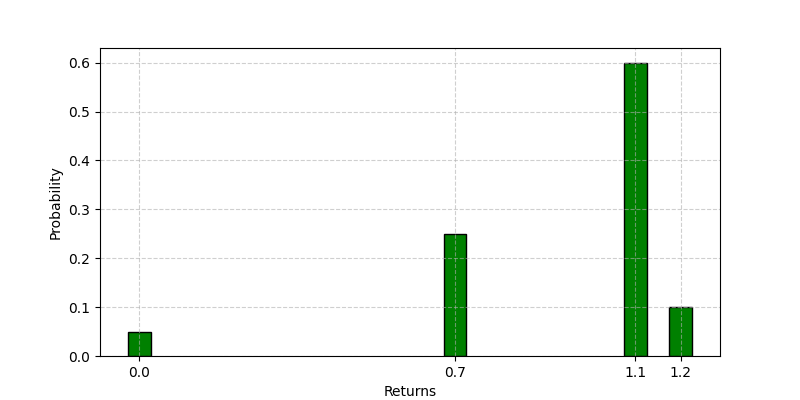
\includegraphics[width=0.8\textwidth]{randomvariables/fig1.png}
    \caption{Example of a random variable distribution.}
    \label{fig:randomvariable}
\end{figure}

Another way to think of a random variable is as a
\textit{function} that maps "states of the world" to
real numbers. For example, the random variable in 
Table \ref{tab:randomvariable} could be:

\begin{table}[!htbp]
    \centering
    \begin{tabular}{c c c}
        % \hline
        $R$ & States of the world & $\pi$ \\
        % \hline
        1.1 & New product works, competitor burns down & 0.6 \\
        1.2 & New product works, competitor ok. & 0.1 \\
        0.7 & Only old products work & 0.25 \\
        0.0 & Factory burns down, no insurance. & 0.05 \\
    \end{tabular}
    \caption{Random variable as a function mapping states of the world to real numbers.}
    \label{tab:statesoftheworld}
\end{table}

The probability really describes the external events 
that define the states of the world. Usually, we 
can't name those events, so we just use the probabilities
that the stock return takes on various values.

In the end, all random variables have a discrete number of values,
as in our example. Stock prices are only listed to 
1/8 dollar, all payments are rounded to the nearest cent, etc.
However, we often think of \textit{continuous} random variables,
that can be any real number. 
Corresponding to the discrete probabilities above,
we now have a continuous probability \textit{density},
usually denoted $f(R)$. 
The density tells you the probability per unit of $R$.
For example, $f(R_0)\Delta R$ tells you the probability
that the return is between $R_0$ and $R_0 + \Delta R$.

A common assumption is that returns (or log returns) are 
normally distributed. This means that the density is
given by the formula:

\begin{equation}
    f(R) = \frac{1}{\sqrt{2\pi\sigma^2}}\exp\left(-\frac{(R-\mu)^2}{2\sigma^2}\right)
\end{equation}

The graph of this function looks like this:
\begin{figure}[!htbp]
    \centering
    \begin{tikzpicture}
        \begin{axis}[
            axis lines=middle,
            xlabel={$R$},
            ylabel={$f(R)$},
            xtick=\empty,  % Removes x ticks
            ytick=\empty,  % Removes y ticks
            enlargelimits,
            clip=false,
            domain=0.8:1.2,  % Adjusted domain to focus around the mean
            samples=100,
            ymin=0,
            ymax=9,  % Adjusted y-max for better visibility
        ]
        % Normal distribution parameters mu and sigma
        \def\mucomp{1}
        \def\sigmacomp{0.05}
        % Normal distribution formula
        \addplot[blue, thick] {1/(sqrt(2*pi*\sigmacomp^2)) * exp(-((x-\mucomp)^2)/(2*\sigmacomp^2))};
        
        % Adding mu label
        \node[pin={[pin edge={thick}, pin distance=0mm]90:{$\mu$}}] at (axis cs:\mucomp, 0) {};
    
        % Highlighting the spread influenced by sigma
        \draw[red, thick, <->] (axis cs:\mucomp-\sigmacomp,5) -- (axis cs:\mucomp+\sigmacomp,5)
            node[pos=0.5, fill=white] {$\sigma$};
    
    \end{axis}
    \end{tikzpicture}
    \caption{The probability density function of normally distributed returns}
\end{figure}

About $30\%$ ($31.73\%$ to be exact) of the probability 
of a normal distribution is more than one standard deviation
away from the mean. About $5\%$ of the probability is more
than two standard deviations away from the mean (in fact 
$4.55\%$, the $5\%$ probability lines is at 1.96 standard deviation).
That means that there is only one chance in 20 that the return
will be more than two standard deviations away from the mean 
in a normally distributed world. In reality, stock returns 
have "fat tails", meaning that they are more likely to take 
on extreme values than a normal distribution would suggest.

You can experiment modelling returns with
a normal distribution in Python:

\begin{python}
import numpy as np

# Parameters for the normal distribution
mu = 1  # Mean
sigma = 0.05  # Standard deviation

print(np.random.normal(mu, sigma, 1))
\end{python}

\section{Expected Value and Variance of Returns}

Rather than plot the entire distribution, 
we usually summarize the behavior of a random variable
with two numbers: the \textit{mean} and the
\textit{variance}.

We denote the values that $R$ can takes on a $R_i$, 
with associated probabilities $\pi_i$. 
The mean of $R$ is given by:

\begin{equation}
    E(R) = \sum_i R_i \pi_i
\end{equation}

The mean is a measure of \textit{central tendency}.
It tells you where $R$ is on average. A high mean
stock return is obviously better than a low mean
stock return.

The \textit{variance} of $R$ is given by:

\begin{equation}
    \sigma^2(R) = E[(R - E(R))^2]
    = \sum_i \pi_i(R_i - E(R))^2
\end{equation}

Since squares are always positive, variance tells 
you how much $R$ is far away from its mean. It 
measures the spread of the distribution. High 
variance is not a good thing. It will be 
our measure of \textit{risk}.

Using our previous example, the Python code is:

\begin{python}
import numpy as np

# Define the values that R can take (R_i) and their associated probabilities (pi_i)
values = np.array([1.1, 1.2, 0.7, 0.0])  # Example values R_i
probabilities = np.array([0.6, 0.1, 0.25, 0.05])  # Corresponding probabilities pi_i

# Calculate the expected value (mean) of R
expected_value = np.sum(values * probabilities)
print("Expected Value E(R):", expected_value)

# Calculate the variance of R
variance = np.sum((values - expected_value)**2 * probabilities)
print("Variance of R:", variance)

\end{python}


The \textit{covariance} is:

\begin{equation}
    \text{Cov}(R^a, R^b) = E[(R^a - E(R^a))(R^b - E(R^b))]
    = \sum_{i} \pi_{i}[(R^a_i - E(R^a))(R^b_i - E(R^b))]
\end{equation}

It measures the tendency of two returns to move 
together. It's positive if they tend to move in the 
same direction, negative if one tends to go up when
the other goes down. It's zero if they are independent.

The size of the covariance depends on the unit 
of measurement. For example, if we measure 
one return in cents, the covariance goes up by 
a factor of 100, even though the relationship
between the two returns is the same. The 
\textit{correlation coefficient} resolves this problem:

\begin{equation}
    \text{Corr}(R^a, R^b) = \frac{\text{Cov}(R^a, R^b)}{\sigma(R^a)\sigma(R^b)}
\end{equation}

The correlation coefficient is always between -1 and 1.

Keeping the same example as before but adding a second return, 
the Python code is:

\begin{python}
import numpy as np

# Define the values and probabilities for two random variables R^a and R^b
values_a = np.array([1.1, 1.2, 0.7, 0.0])  # Example values R^a_i
values_b = np.array([1.0, 1.3, 0.4, 0.1])  # Example values R^b_i
probabilities = np.array([0.6, 0.1, 0.25, 0.05])  # Corresponding probabilities pi_i

# Calculate the expected values (means) of R^a and R^b
expected_value_a = np.sum(values_a * probabilities)
expected_value_b = np.sum(values_b * probabilities)

# Calculate the covariance between R^a and R^b
covariance = np.sum(probabilities * (values_a - expected_value_a) * (values_b - expected_value_b))
print("Covariance between R^a and R^b:", covariance)

# Calculate the variances of R^a and R^b
variance_a = np.sum((values_a - expected_value_a)**2 * probabilities)
variance_b = np.sum((values_b - expected_value_b)**2 * probabilities)

# Calculate the standard deviations of R^a and R^b
std_dev_a = np.sqrt(variance_a)
std_dev_b = np.sqrt(variance_b)

# Calculate the correlation coefficient
correlation_coefficient = covariance / (std_dev_a * std_dev_b)
print("Correlation Coefficient between R^a and R^b:", correlation_coefficient)
\end{python}

\section{Returns Algebra}

We will have to do a lot of manipulation of random variables. 
For example, we will want to know what is the mean 
and standard deviation of a \textit{portfolio} of 
two returns. To derive any of these rules, we have to keep in mind
 the definitions in the previous section.

First interesting fact: constants come out of 
expectations and expectations of sums are equals 
to sums of expectations. For example, if $c$ and $d$
are real numbers:

\begin{equation}
    E(cR^a) = cE(R^a)
\end{equation}

\begin{equation}
    E(R^a + R^b) = E(R^a) + E(R^b)
\end{equation}

\begin{equation}
    E(cR^a + dR^b) = cE(R^a) + dE(R^b)
\end{equation}

Let's check this with Python:

\begin{python}
import numpy as np

# Define the values for random variable R^a and its associated probabilities
values_a = np.array([1.1, 1.2, 0.7, 0.0])  # Example values R^a_i
probabilities = np.array([0.6, 0.1, 0.25, 0.05])  # Corresponding probabilities pi_i

# Calculate the expected value of R^a
expected_value_a = np.sum(values_a * probabilities)
print("Expected Value E(R^a):", expected_value_a)

# Define the constant c
c = 0.5

# Calculate the expected value of cR^a using the definition
expected_value_cRa = np.sum(c * values_a * probabilities)
print("Expected Value E(cR^a):", expected_value_cRa)

# Calculate c times the expected value of R^a
c_times_expected_value_a = c * expected_value_a
print("c * E(R^a):", c_times_expected_value_a)

# Check if E(cR^a) is numerically equal to cE(R^a)
if np.isclose(expected_value_cRa, c_times_expected_value_a):
    print("Numerically verified that E(cR^a) = cE(R^a)")
else:
    print("Numerical discrepancy found")
\end{python}

Variance of sums works like taking a square:

\begin{equation}
    \sigma^2(R^a + R^b) = \sigma^2(R^a) + \sigma^2(R^b) + 2\text{Cov}(R^a, R^b)
\end{equation}

With constants $c$ and $d$:	

\begin{equation}
    \sigma^2(cR^a + dR^b) = c^2\sigma^2(R^a) + d^2\sigma^2(R^b) + 2cd\text{Cov}(R^a, R^b)
\end{equation}

The covariance works linearly with constants:

\begin{equation}
    \text{Cov}(cR^a, dR^b) = cd\text{Cov}(R^a, R^b)
\end{equation}

In Python:

\begin{python}
import numpy as np

# Define the values and probabilities for two random variables R^a and R^b
values_a = np.array([1.1, 1.2, 0.7, 0.0])  # Example values R^a_i
values_b = np.array([1.0, 1.3, 0.4, 0.1])  # Example values R^b_i
probabilities = np.array([0.6, 0.1, 0.25, 0.05])  # Corresponding probabilities pi_i

# Calculate the expected values (means) of R^a and R^b
expected_value_a = np.sum(values_a * probabilities)
expected_value_b = np.sum(values_b * probabilities)

# Calculate the covariance between R^a and R^b
covariance_ab = np.sum(probabilities * (values_a - expected_value_a) * (values_b - expected_value_b))
print("Covariance Cov(R^a, R^b):", covariance_ab)

# Constants c and d
c = 0.5  # Scaling factor for R^a
d = 0.8  # Scaling factor for R^b

# Calculate the covariance between cR^a and dR^b
covariance_cRa_dRb = np.sum(probabilities * (c * (values_a - expected_value_a)) * (d * (values_b - expected_value_b)))
print("Covariance Cov(cR^a, dR^b):", covariance_cRa_dRb)

# Calculate cd * Cov(R^a, R^b)
cd_covariance_ab = c * d * covariance_ab
print("cd * Cov(R^a, R^b):", cd_covariance_ab)

# Check if Cov(cR^a, dR^b) is numerically equal to cd * Cov(R^a, R^b)
if np.isclose(covariance_cRa_dRb, cd_covariance_ab):
    print("Numerically verified that Cov(cR^a, dR^b) = cd * Cov(R^a, R^b)")
else:
    print("Numerical discrepancy found")
\end{python}

Normal distributions have an extra property. 
Linear combinations of normally distributed random variables 
are again normally distributed. 
Precisely, if $R^a$ and $R^b$ are normally distributed and:

\begin{equation}
    R^p = cR^a + dR^b
\end{equation}

then $R^p$ is normally distributed. 

A variable $R$ is \textit{lognormally} distributed 
if $r := \ln(R)$ is normally distributed.
This is a nice model for stock returns since you 
can never lose more than all your money (\textit{i.e.}
you can never see $R < 0$). A lognormal distribution
captures this property.
A normal distribution always includes events 
in which $R < 0$, which is not possible for stock returns.

\section{Sample Returns}

So far, we have worked as if we knew the probabilities
of each return. In reality, we don't. We have to
\textit{estimate} them from \textit{sample returns}.
Similarly, if we don't know the mean, variance, regression
coefficients, etc., we have to estimate them as well.
That's what \textit{statistics} is about.

The \textit{average} or \textit{sample mean} is:

\begin{equation}
    \bar{R} = \frac{1}{T}\sum_{i=1}^N R_t
\end{equation}

where $\{R_0, R_1, \ldots, R_{T}\}$ is a \textit{sample}
of data on a stock returns. We need to keep the 
\textit{sample mean} and the true, or \textit{population mean}
separate in our heads. For example, the true 
probabilities that a coin will lands heads is $0.5$, 
so the mean of a bet on a coin toss (1\$ if heads, -1\$ if tails)
is $0.5 \times 1 + 0.5 \times -1 = 0$.
A \textit{sample} of coin tosses might be $\{H, T, H, H, T\}$,
In that \textit{sample}, the frequency of heads is $3/5 = 0.6$ and 
the frequency of tails is $2/5 = 0.4$. So the \textit{sample mean}
of a coin toss bet is $0.6 \times 1 + 0.4 \times -1 = 0.2$.

As the sample gets bigger, the \textit{sample mean} 
will gets closer to the \textit{population mean}. 
That property of the sample mean is called \textit{consistency}.
It makes it a good estimator of the population mean.
But the sample and population mean are not the same thing 
for any finite sample.

Also, sample means approach population means only if 
you are repeatedly doing the same thing, like tossing
a fair coin. This may not be true for stock returns. 
If there are days when expected returns are high and
days when they are low, then the average return 
will not necessarily recover the expected return.

The \textit{sample variance} is:

\begin{equation}
    s^2 = \hat{\sigma}^2 = \frac{1}{T - 1}\sum_{i=1}^T (R_t - \bar{R})^2
\end{equation}

The sample mean and sample variance vary from sample to sample.
Let's flip a coin, with $Heads = +1$ and $Tails = -1$.
If we get $\{H, T, H, H, T\}$, the sample mean is 
$0.2$, but if we get $\{H, H, H, H, H\}$, the sample mean is $1$.
The true population mean, of course, is $0$.
Thus, the sample mean, the standard deviation, and other 
statistics are also \textit{random variables}, as 
they vary from sample to sample.
They are random variables that depends on the whole sample, 
not just what happened one day, but they are random variables
nonetheless. The population mean and variance are just 
numbers. 

We can then ask, "how much does the sample mean vary from
sample to sample?" If a mutual fund manager tells you
that his fund has a mean return of $10\%$ while the 
market has a mean return of $8\%$, you want to know 
if it was just luck or if it means that his true,
population mean, which you are likely to earn in the 
next 5 years, is $2\%$ higher than the market.
In other words, was the \textit{realization} of the
random variable called "my estimate of manager A's 
mean return" near the mean of the true or population mean
of the random variable called "manager A's return"?

Figuring out the variation of the sample mean is 
a good use of statistics. The sample mean is:

\begin{equation}
    \bar{R} = \frac{1}{T}\sum_{i=1}^T R_t
\end{equation}

Therefore,

\begin{equation}
    E(\bar{R}) = \frac{1}{T}\sum_{i=1}^T E(R_t) = E(R)
\end{equation}

assuming all the $R_t$ are drawn from the same distribution.
This verifies that the sample mean is \textit{unbiased}.
On average, across many samples, the sample mean 
will reveal the true mean. The variance of the sample mean is:

\begin{equation}
    \sigma^2(\bar{R}) = \sigma^2(\frac{1}{T}\sum_{i=1}^T R_t) 
    = \frac{1}{T^2}\sum_{i=1}^T \sigma^2(R_t) + \text{covariance terms}
\end{equation}

If we assume that all the covariances are zero ($R_t$ are 
independent), then the variance of the sample mean is:

\begin{equation}
    \sigma^2(\bar{R}) = \frac{1}{T}\sigma^2(R)
\end{equation}

and the standard deviation:

\begin{equation}
    \sigma(\bar{R}) = \frac{1}{\sqrt{T}}\sigma(R)
\end{equation}

For stock returns, $\text{Cov}(R_t, R_{t+1}) = 0$ 
is a good assumption. It's a great assumption for 
coin tosses: seeing heads this time makes not 
more likely to see heads next time. 

We don't know $\sigma$. We have to \textit{estimate}
the sampling variation of the sample mean by using 
your estimate of $\sigma$, namely the sample standard
deviation. If we use hats to denote estimate:

\begin{equation}
    \hat{\sigma}(\bar{R}) = \frac{1}{\sqrt{T}}\hat{\sigma}(R)
\end{equation}

The classic use of this formula is to give a standard error
or measure of uncertainty of the sample mean, and 
to test whether the sample mean is equal to some value,
usually zero. 

The test is based on a \textit{condifence interval}. 
Assuming normal distribution, the confidence interval 
for the mean is the sample mean plus or minus 2 (in fact 1.96)
standard errors. The meaning of this interval 
is that if the true mean was outside the interval, 
there would be less than $5\%$ chance of seeing a 
sample mean as high or low as the one you got.

There is an easier method. We can just calculate the
probability that the sample mean comes out at its 
actual value (or higher) given the null hypothesis,
\textit{i.e.} calculate the area under the distribution 
of the sample mean past the sample mean we have,
given an assumption (hypothesis) about the true mean.
This is the \textit{p-value}.

Usually, tests are run using the \textit{t-distribution}.
When you take account of sampling variation in $\hat{\sigma}$,
you can show that the ratio:

\begin{equation}
    \sqrt{T}\frac{\bar{R} - E(R)}{\hat{\sigma}}
\end{equation}

is not a normal distribution with mean zero and variance 
one, but a \textit{t-distribution} with $t$ degrees of freedom.


\section{Conclusion}

\newpage
\section{Exercises}

\subsection{}

Compute the expected return $E(R)$ for the 
$R = [1.1, 1.2, 0.7, 0.0]$ with probabilities
$\pi = [0.6, 0.1, 0.25, 0.05]$ with Python.

\subsection{}

Derive $E(cR^a) = cE(R^a)$ using the 
definition of expectations $E(R) = \sum_i R_i \pi_i$.

\subsection{}

Derive the variance of sums formula:
\begin{equation}
    \sigma^2(R^a + R^b) = \sigma^2(R^a) + \sigma^2(R^b) + 2\text{Cov}(R^a, R^b)
\end{equation}

using the definition of variance $\sigma^2(R) = E[(R - E(R))^2]$ and
the definition of covariance $\text{Cov}(R^a, R^b) = E[(R^a - E(R^a))(R^b - E(R^b))]$.



\subsection{}

Express the expected return $E(R^p)$ 
and variance $\sigma^2(R^p)$ of the
portfolio $R^p$ with returns $R^a$ and $R^b$
and weights $c$ and $d$.

\newpage
\section{Solutions}

\subsection{}

\begin{python}
import numpy as np

# Define the returns and their corresponding probabilities
returns = np.array([1.1, 1.2, 0.7, 0.0])  # Values of R
probabilities = np.array([0.6, 0.1, 0.25, 0.05])  # Corresponding probabilities pi

# Calculate the expected return E(R)
expected_return = np.sum(returns * probabilities)
print("Expected Return E(R):", expected_return)
\end{python}


\subsection{}

\begin{equation}
    E(cR^a) = \sum_i \pi_i c R^a_i  = c\sum_i  \pi_i R^a_i = cE(R^a)
\end{equation}

\subsection{}

\begin{align}
    \sigma^2(R^a + R^b) &= E[(R^a + R^b - E(R^a + R^b))^2] \\
    &= E[(R^a + R^b - E(R^a) - E(R^b))^2] \\
    &= E[(R^a - E(R^a) + R^b - E(R^b))^2] \\
    &= E[(R^a - E(R^a))^2 + (R^b - E(R^b))^2 + 2(R^a - E(R^a))(R^b - E(R^b))] \\
    &= \sigma^2(R^a) + \sigma^2(R^b) + 2\text{Cov}(R^a, R^b)
\end{align}

\subsection{}

Its mean is:

\begin{equation}
    E(R^p) = cE(R^a) + dE(R^b)
\end{equation}

and its variance is:

\begin{equation}
    \sigma^2(R^p) = c^2\sigma^2(R^a) + d^2\sigma^2(R^b) + 2cd\text{Cov}(R^a, R^b)
\end{equation}